\graphicspath{ {images/2_source_localization/} }
\chapter{Sound Source Localization}
\section{Physical background}
This section shows some underling fundamentals on which the following described theory is based on.
\todo{Schribe}

\section{Sound Source Localization Methods}
\acrfull{ssl} \todo{Abbr Verzwichnis} is a well researched area with many applications.
\cite{nat_skript}
The basic system can be brought into two categories, time based or power based methods.
\subsection{Power based \acrshort{ssl}}
The idea of power based SSL is based of the known propagation properties of sound waves in air.
BlaBlaBla \todo{short text}
However for this method to work some properties of the sound source have to be known.
Additionally the sensors that measure the sound power levels have to be calibrated \dots

\subsection{Time Based \acrshort{ssl}}
Another group of \acrshort*{ssl} is based on the time when the
signal is received by the microphones.
Given a source at a location $S = (x_S,y_S)^T$ and $N$ microphones at locations
$M_n = (x_n,y_n)^T$ the time it takes for a accoustic signal from the source to reach a microphone is
\begin{equation}
  t_n = \frac{\lVert S - M_n\rVert}{c}
  = \frac{\sqrt{\left(x_S - x_n\right) + \left(y_S - y_n\right)}}{c} .
\end{equation}
So if $t_n$ is known for a microphone, the location of the source can be limited to point on a circle
around $M_n$ with a radius of $t_n c$.
\todo{Differences}

\begin{figure}
  \centering
  \begin{subfigure}[b]{0.45\textwidth}
    \centering
    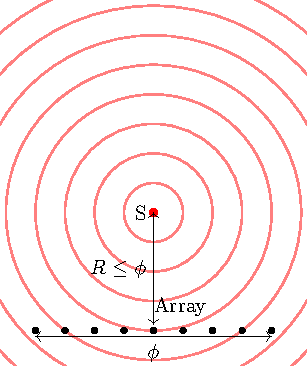
\includegraphics[width=\textwidth]{NearField.pdf}
    \caption{Near-Field Case}
    \label{fig:y equals x}
  \end{subfigure}
  \hfill
  \begin{subfigure}[b]{0.45\textwidth}
    \centering
    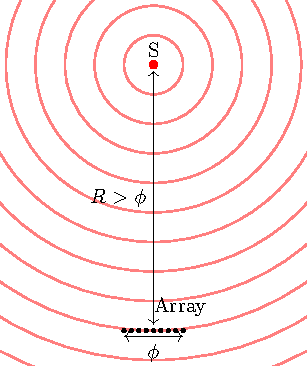
\includegraphics[width=\textwidth]{FarField.pdf}
    \caption{Far-field Case}
    \label{fig:three sin x}
  \end{subfigure}
  \caption{Three simple graphs}
  \label{fig:three graphs}
\end{figure}



\begin{figure}
  \centering
  %    \includegraphics[width=0.25\textwidth]{mesh}
  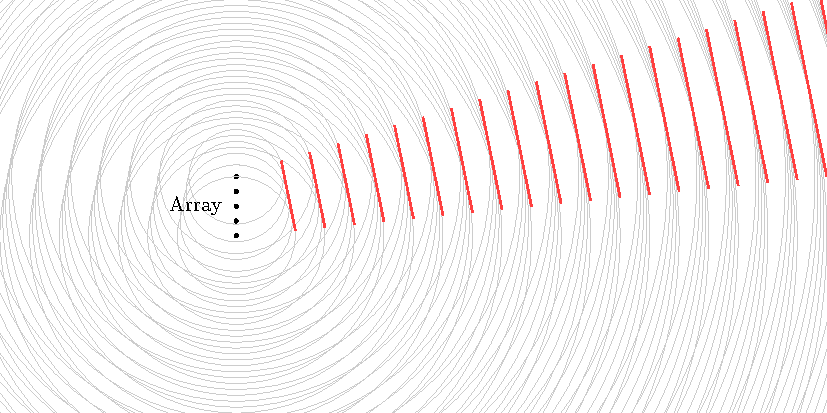
\includegraphics[]{beamforming_1.pdf}
  \caption{a nice plot}
  \label{fig:mesh1}
\end{figure}

\newpage
\section{Simulator}
Blabla
